\section{Overall Description}

\subsection{Product Perspective}
Here we discuss in details all the shared phenomena outlined in the previous section, and we provide an oversight of the domain model in different levels of specification, by means of class and state diagrams. \\ \\
\noindent
\textbf{Registration/Login} (world controlled, machine observed)\\
The User can submit his/her credentials in order to register or log in if is already registered. The application provides a minimal and intuitive form which, once filled and submitted, collects, checks and then sends all the data to the associated DBMS. \\ 

\noindent
\textbf{Manage events} (world controlled, machine observed)\\
The User is able through the calendar to add, edit or delete events from the schedule. In the first two cases, the System will check if the information inserted in the fields are consistent and complete and will send them to the DBMS.  \\

\noindent
\textbf{Set travel preferences} (world controlled, machine observed)\\
The User is able to customize his/her travel means preferences in the homonym section provided by the System. Here, every mean has a specific tab with a list of applicable constraints. The User can also globally activate/deactivate a particular travel mean. The application will store all the preferences selected by the User and will use them to suggest the best travel options.  \\

\noindent
\textbf{Suggest travel options} (machine controlled, world observed)\\
When the User adds or edits an event, the System shows up all the possible traveling options computed according to the specified preferences. The User can then select one of them. \\

\noindent
\textbf{Generate warnings} (machine controlled, world observed)\\
When a User tries to add a new event to the daily schedule, the System computes a study of feasibility to check if it creates any schedule conflict. If it does, the System will display a warning message to advise the User that the new event cannot deal with the previous ones and the event won't be added to the schedule. \\

\noindent
\textbf{Send notifications} (machine controlled, world observed)\\
If the notification option is enabled, the System will advise the User through an alert message. The System computes the instant to send the notification according to its internal clock.\\

\subsubsection{Class Diagram}

\begin{figure}[H]
	\centering
	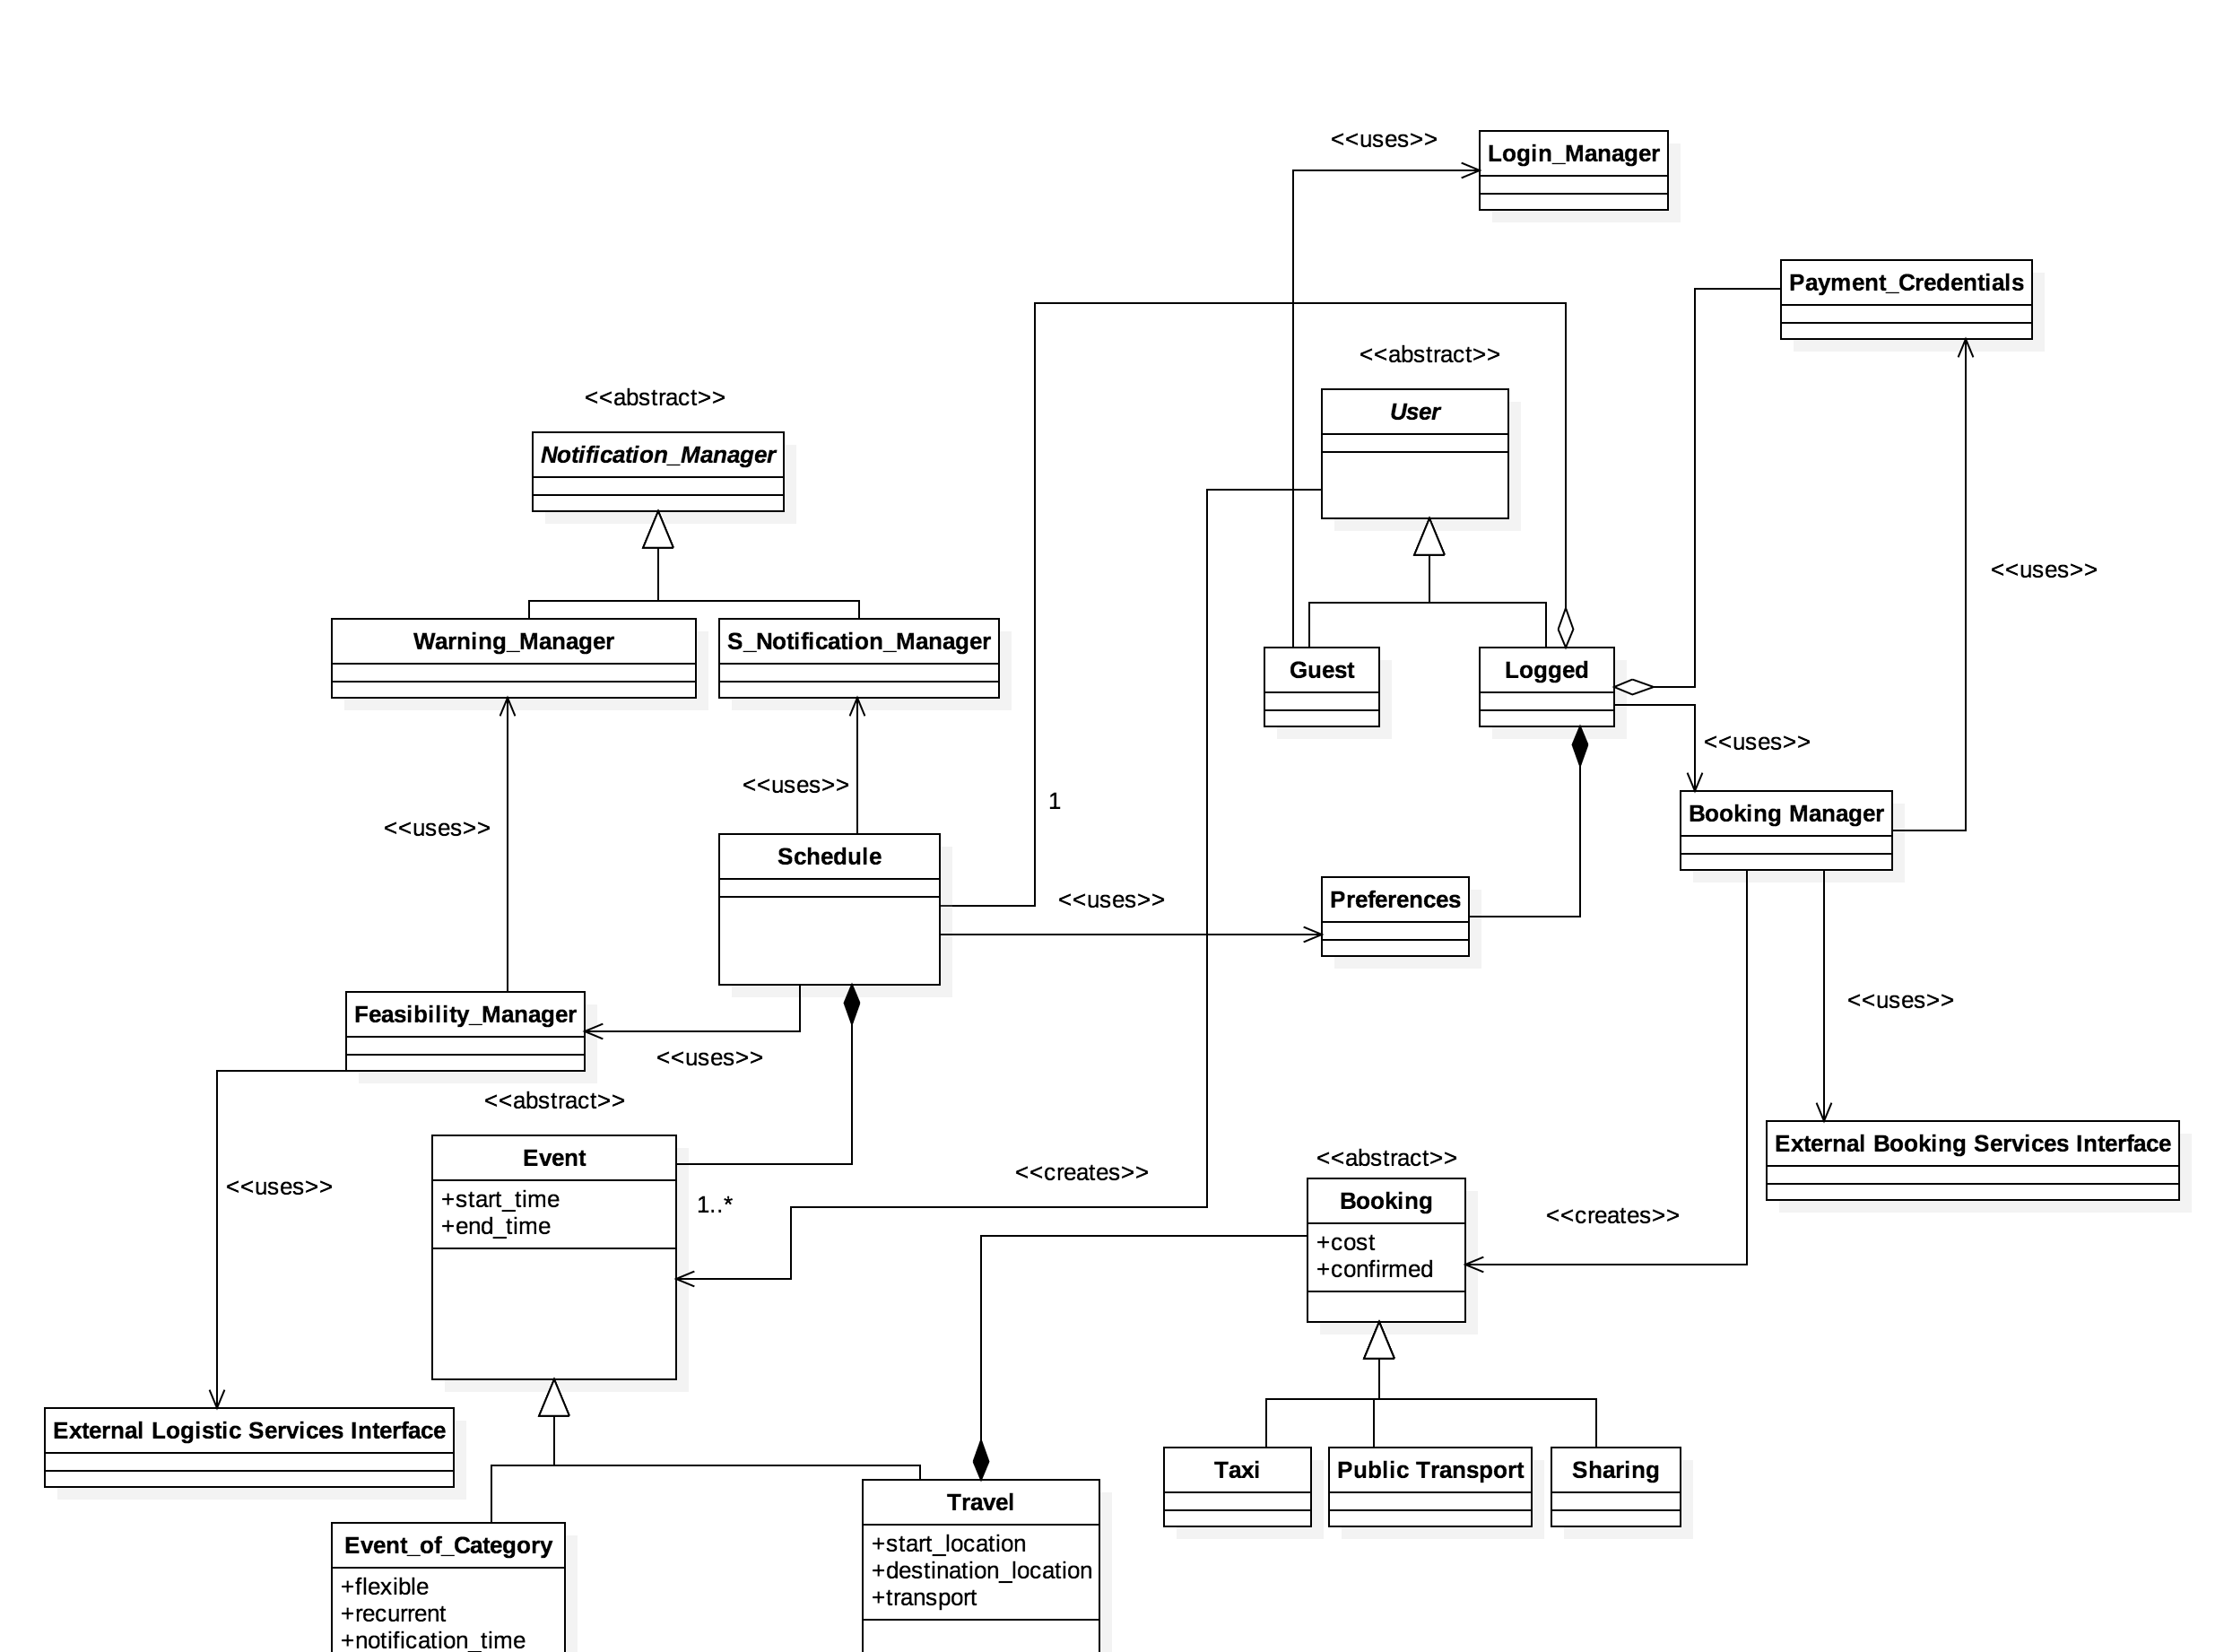
\includegraphics[width=1\textwidth]{classdiagram}
	\caption{\textit{Travlendar+} Class Diagram}
\end{figure}

\subsubsection{State Chart Diagrams}

\begin{figure}[H]
	\centering
	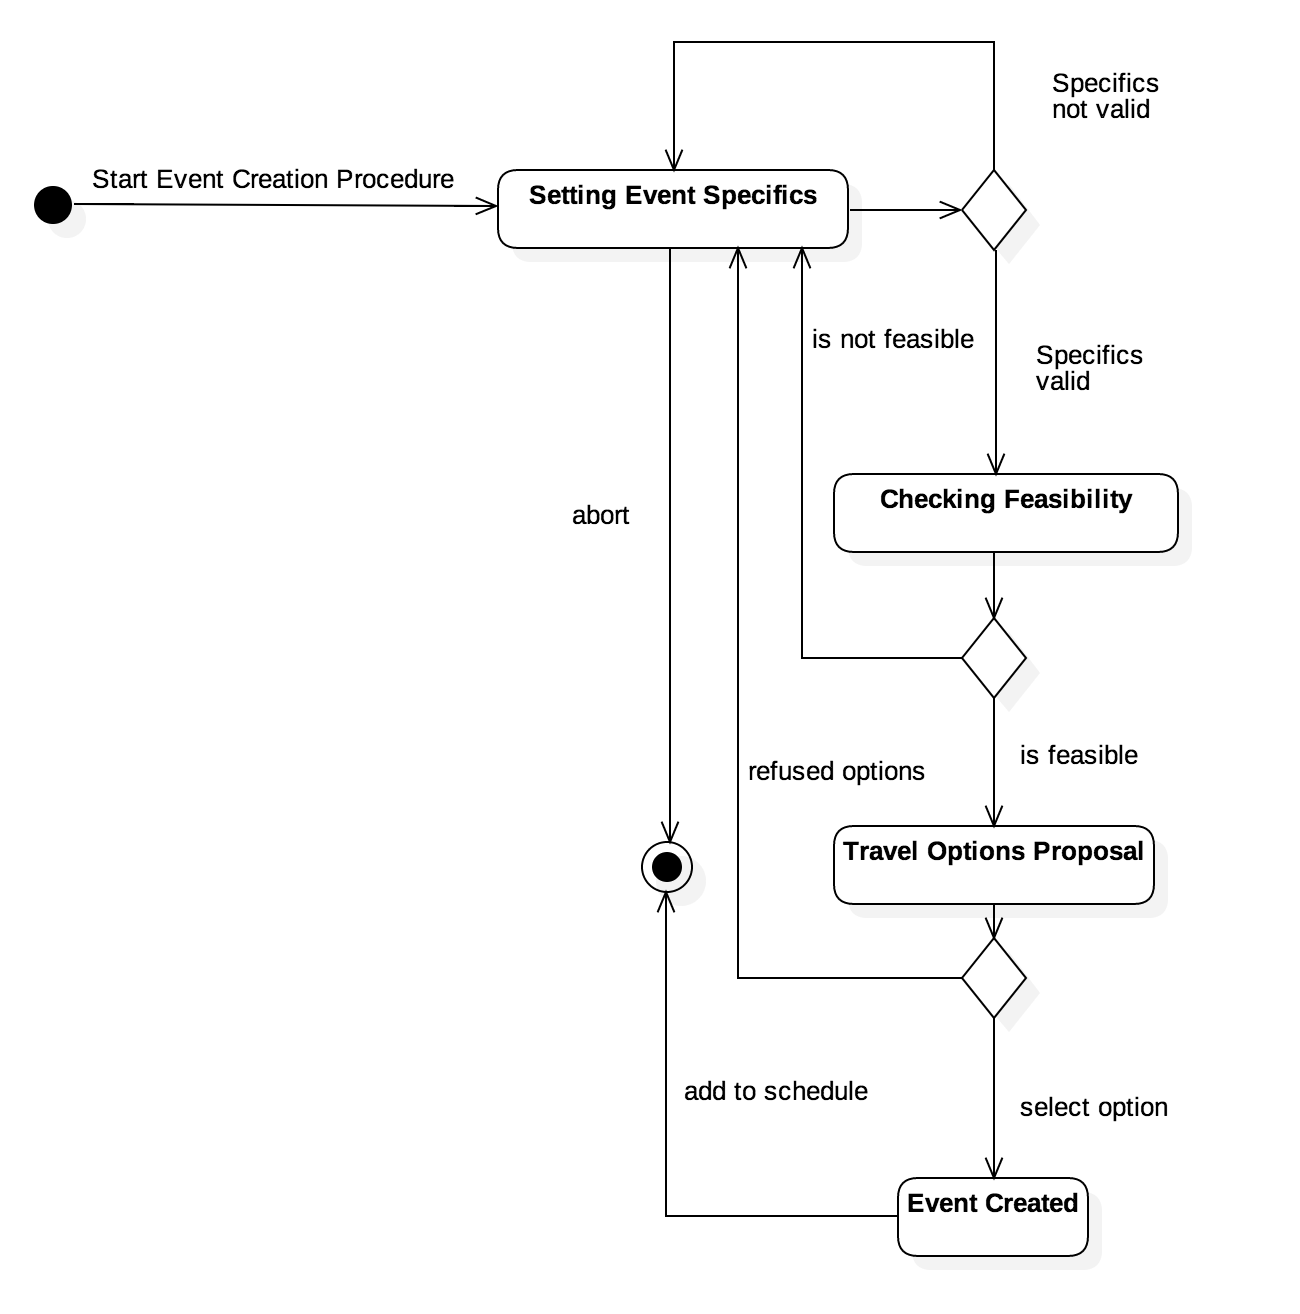
\includegraphics[width=1\textwidth]{eventadd}
	\caption{Add event state chart}
\end{figure}

\begin{figure}[H]
	\centering
	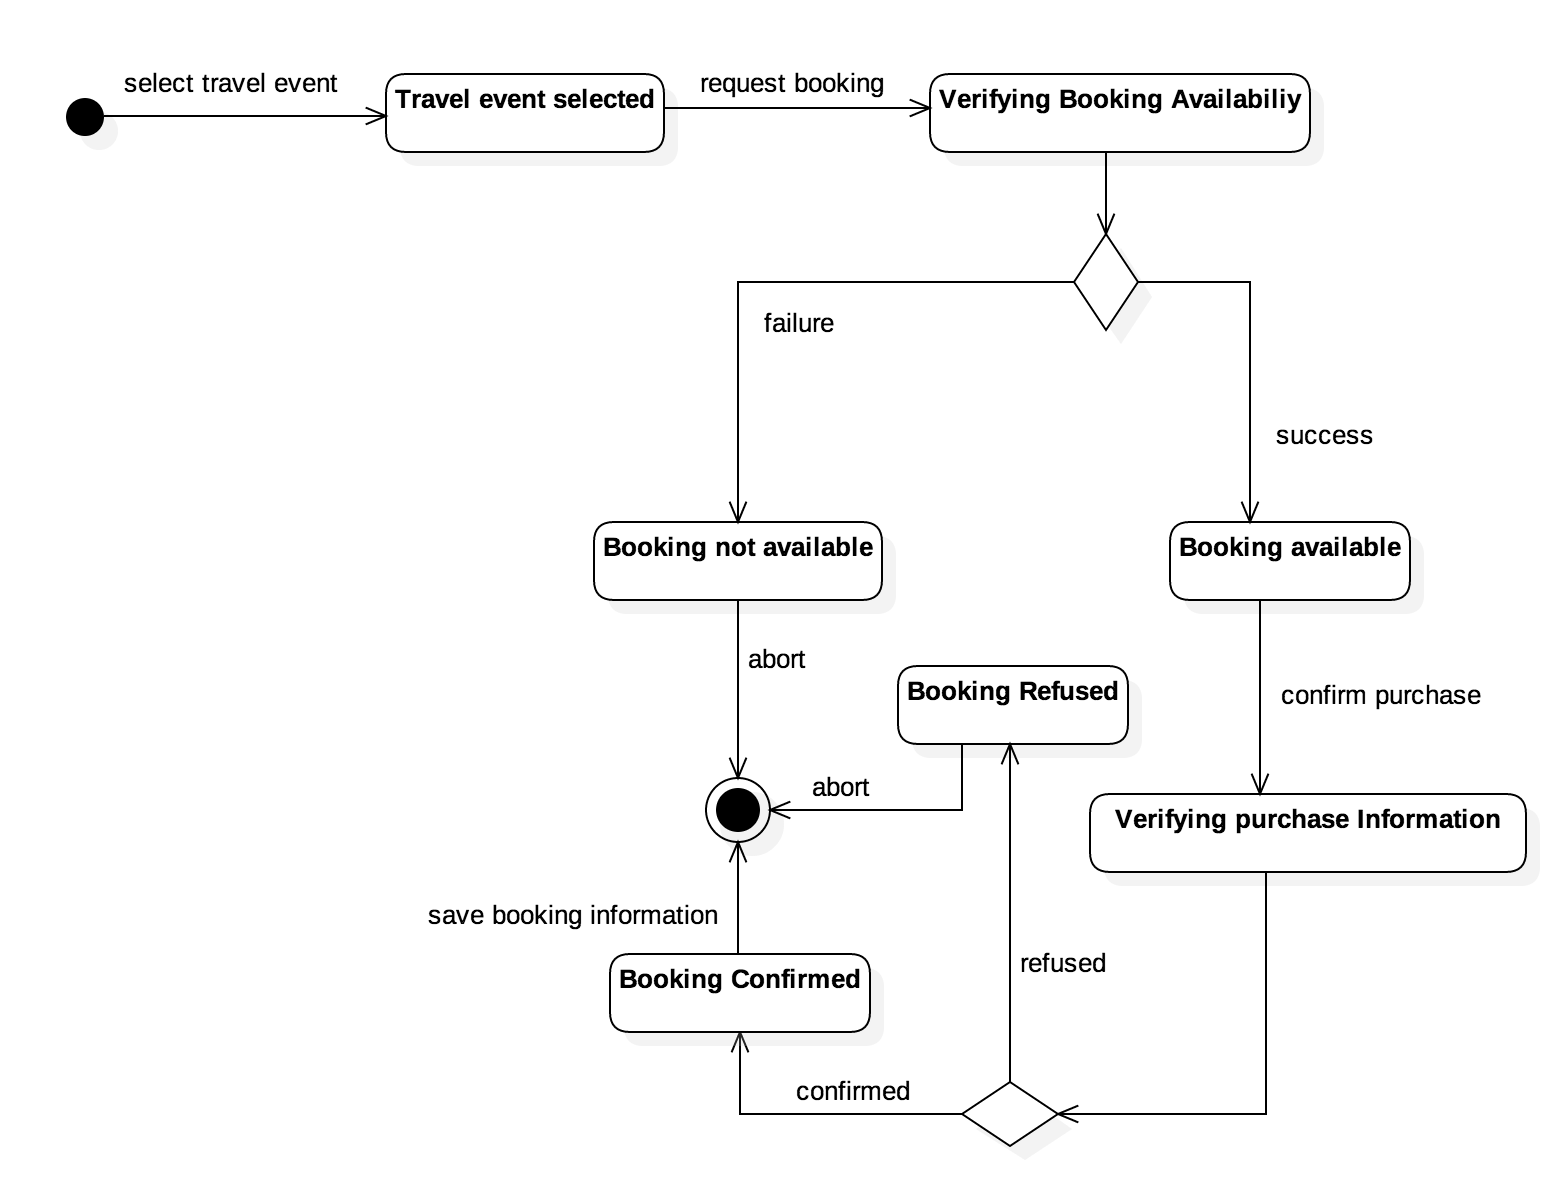
\includegraphics[width=1\textwidth]{booktravel}
	\caption{Booking travel state chart}
\end{figure}

\newpage
\subsubsection{Use Case Diagrams}

\begin{figure}[H]
	\centering
	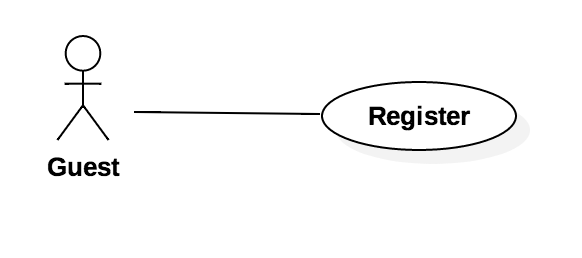
\includegraphics[width=0.5\textwidth]{actorguest}
	\caption{Guest use case}
\end{figure}

\begin{figure}[H]
	
	\centering
	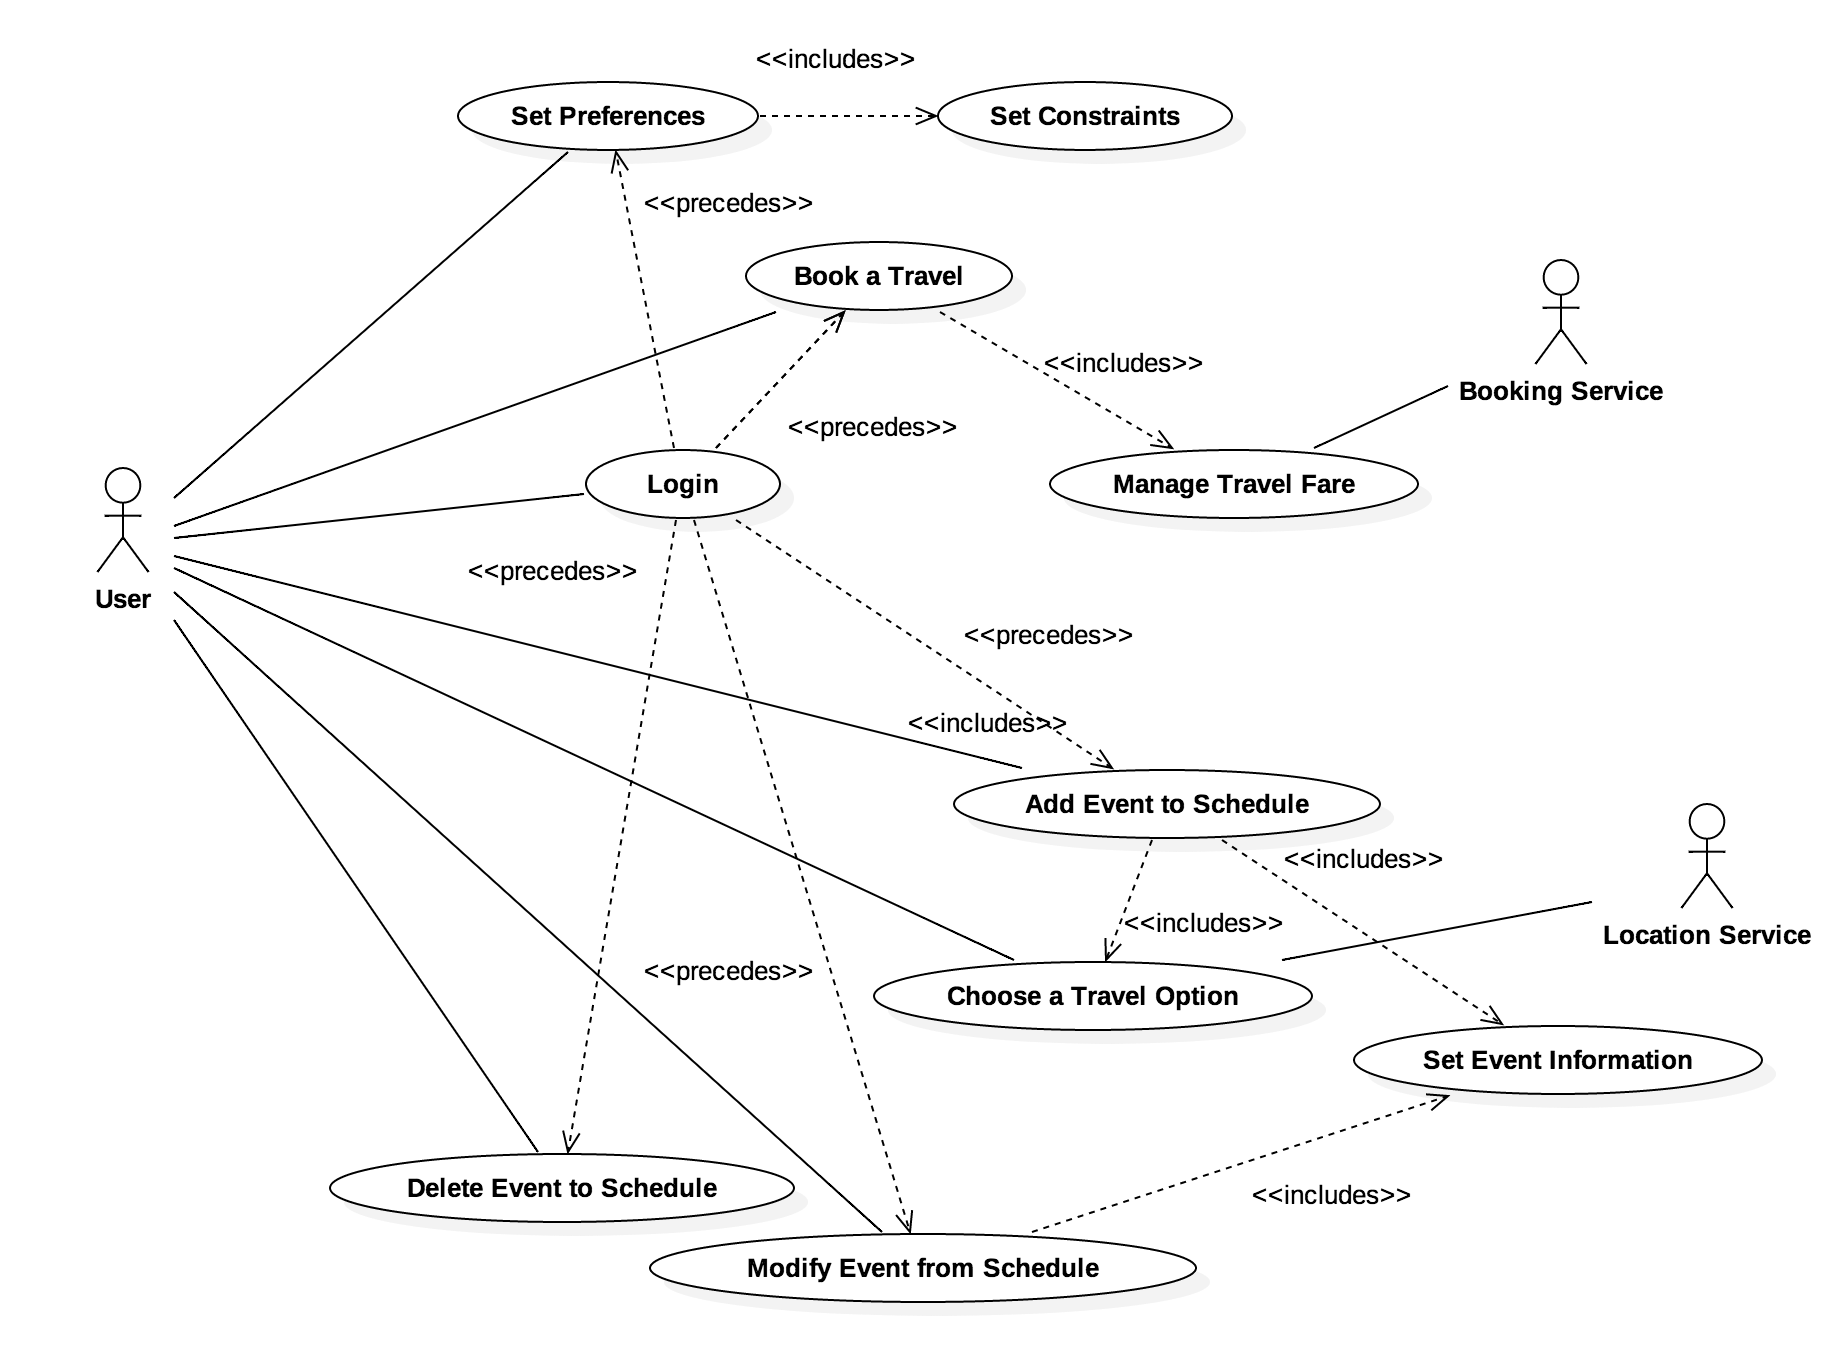
\includegraphics[width=1\textwidth]{actoruser}
	\caption{User use case}
\end{figure}

\newpage
\subsubsection{Use Case Templates}
\begin{center}
	\textbf{Register Account}
\end{center}

\begin{tabularx}{\linewidth}{| l | X |}
	\hline
	\textbf{ID} & UC1\\
	
	\hline
	\textbf{Description} & The \textbf{\textit{Guest}} wants to create an account for the application.\\
	
	\hline
	\textbf{Actors} & \textbf{\textit{Guest}}\\
	
	\hline
	\textbf{Preconditions} & The \textbf{\textit{Guest}} opened the application\\
	
	\hline
	\textbf{Flow of Events} & \parbox{0.7\textwidth}{\begin{enumerate}
			\item The \textbf{\textit{Guest}} selects the function \textit{Sign Up}.
			\item The \textbf{\textit{System}} returns a form to enter all the required data: username, email address and password which will be used for the future logins.
			\item The \textbf{\textit{Guest}} fills the form with all the required information.
			\item The \textbf{\textit{User Manager}} checks if all the informations are correct, generates a random activation URL and asks the \textbf{\textit{Mailing System}} to forward his/her URL to the email address of the \textbf{\textit{Guest}}.
			\item The \textbf{\textit{Guest}} receives the mail and click on the URL. The \textbf{\textit{User Manager}} stores the data provided by the \textbf{\textit{User}}.
	\end{enumerate}}\\
	
	\hline
	\textbf{Postconditions} & The \textbf{\textit{Guest}} is able to sign in.\\
	
	\hline
	\textbf{Exceptions} & \parbox{0.7\textwidth}{ \begin{enumerate}
			\item The \textbf{\textit{User Manager}} recognizes invalid information than shows an error message. The flow restarts from point 2.
		\end{enumerate}}\\
	
	\hline
	
\end{tabularx}
\newpage
\begin{center}
	\textbf{Log In}
\end{center}

\begin{tabularx}{\linewidth}{| l | X |}
	\hline
	\textbf{ID} & UC2\\
	
	\hline
	\textbf{Description} & The \textbf{\textit{User}} wants to log in to the application.\\
	
	\hline
	\textbf{Actors} & \textbf{\textit{User}}\\
	
	\hline
	\textbf{Preconditions} & The \textbf{\textit{User}} opened the application\\
	
	\hline
	\textbf{Flow of Events} & \parbox{0.7\textwidth}{\begin{enumerate}
			\item The \textbf{\textit{User}} inserts his/her credentials.
			\item The \textbf{\textit{User}} taps the \textit{Sign In} button.
			\item The \textbf{\textit{User Manager}} checks provided credentials.
	\end{enumerate}}\\
	
	\hline
	\textbf{Postconditions} & The \textbf{\textit{User}} is logged in.\\
	
	\hline
	\textbf{Exceptions} & \parbox{0.7\textwidth}{ \begin{enumerate}
			\item The \textbf{\textit{User Manager}} recognizes invalid credentials then shows an error message. The flow restarts from point 2.
	\end{enumerate}}\\
	
	\hline
	
\end{tabularx}

%\begin{center}
%	\textbf{Log out}
%\end{center}
%
%\begin{tabularx}{\linewidth}{| l | X |}
%	\hline
%	\textbf{ID} & UC3\\
%	
%	\hline
%	\textbf{Description} & The \textbf{\textit{User}} wants to log out of the \textbf{\textit{Travlendar+}} application.\\
%	
%	\hline
%	\textbf{Actors} & \textbf{\textit{User}}\\
%	
%	\hline
%	\textbf{Preconditions} & The \textbf{\textit{User}} is logged in to the application.\\
%	
%	\hline
%	\textbf{Flow of Events} & \parbox{0.7\textwidth}{\begin{enumerate}
%			\item The \textbf{\textit{User}} opens the menu.
%			\item The \textbf{\textit{User}} tap the \textit{Log Out} section.
%			\item The \textbf{\textit{Notification Manager}} displays a confirmation message.
%			\item The \textbf{\textit{User}} selects \textit{yes}.
%			\item The \textbf{\textit{System}} performs the \textbf{\textit{User's}} log out.
%	\end{enumerate}}\\
%	
%	\hline
%	\textbf{Postconditions} & The \textbf{\textit{User}} is logged out.\\
%	
%	\hline
%	\textbf{Exceptions} & \parbox{0.7\textwidth}{ \begin{enumerate}
%			\item The \textbf{\textit{User}} selects the \textit{No} option. The flow of events restarts from point 1.
%	\end{enumerate}}\\
%	
%	\hline
%	
%\end{tabularx}

\begin{center}
	\textbf{Set User Settings}
\end{center}

\begin{tabularx}{\linewidth}{| l | X |}
	\hline
	\textbf{ID} & UC4\\
	
	\hline
	\textbf{Description} & The \textbf{\textit{User}} wants to set User settings.\\
	
	\hline
	\textbf{Actors} & \textbf{\textit{User}}\\
	
	\hline
	\textbf{Preconditions} & The \textbf{\textit{User}} is logged in to the application.\\
	
	\hline
	\textbf{Flow of Events} & \parbox{0.7\textwidth}{\begin{enumerate}
			\item The \textbf{\textit{User}} opens the menu.
			\item The \textbf{\textit{User}} taps the \textit{User Settings} section.
			\item The \textbf{\textit{System}} displays the \textit{User Settings} view.
			\item The \textbf{\textit{User}} changes his/her personal informations and clicks the \textit{Confirm} button.
	\end{enumerate}}\\
	
	\hline
	\textbf{Postconditions} & The \textbf{\textit{User}} changed his personal informations.\\
	
	\hline
	\textbf{Exceptions} & \parbox{0.7\textwidth}{\begin{enumerate}
			\item The \textbf{\textit{User Manager}} recognizes invalid credentials then shows an error message. The flow restarts from point 3.
		\end{enumerate}}\\
	
	\hline
	
\end{tabularx}

\begin{center}
	\textbf{Set Travel Preferences}
\end{center}

\begin{tabularx}{\linewidth}{| l | X |}
	\hline
	\textbf{ID} & UC5\\
	
	\hline
	\textbf{Description} & The \textbf{\textit{User}} wants to set travel preferences.\\
	
	\hline
	\textbf{Actors} & \textbf{\textit{User}}\\
	
	\hline
	\textbf{Preconditions} & The \textbf{\textit{User}} is logged in to the application.\\
	
	\hline
	\textbf{Flow of Events} & \parbox{0.7\textwidth}{\begin{enumerate}
			\item The \textbf{\textit{User}} opens the menu.
			\item The \textbf{\textit{User}} taps the \textit{Travel Preferences} section.
			\item The \textbf{\textit{System}} displays the \textit{Travel Preferences} view.
			\item The \textbf{\textit{User}} selects/deselects each travel mean and set specific constraint for the selected ones.
			\item The \textbf{\textit{User}} clicks on the \textit{Confirm} button.
	\end{enumerate}}\\
	
	\hline
	\textbf{Postconditions} & The \textbf{\textit{User}} changed his/her travel preferences. \\
	
	\hline
	\textbf{Exceptions} & \parbox{0.7\textwidth}{}\\
	
	\hline
	
\end{tabularx}

\begin{center}
	\textbf{Add normal and flexible event}
\end{center}

\begin{tabularx}{\linewidth}{| l | X|}
	\hline
	\textbf{ID} & UC6\\
	
	\hline
	\textbf{Description} & The \textbf{\textit{User}} wants to add a normal or flexible event to the schedule.\\
	
	\hline
	\textbf{Actors} & \textbf{\textit{User}}\\
	
	\hline
	\textbf{Preconditions} & The \textbf{\textit{User}} is logged in to the application and is in the \textit{Schedule} or \textit{Calendar} section.\\
	
	\hline
	\textbf{Flow of Events} & \parbox{0.7\textwidth}{\begin{enumerate}
			\item The \textbf{\textit{User}} clicks the \textit{Add} button.
			\item The \textbf{\textit{System}} returns a form to enter all the required data: name, position of the event, previous position (from where the appointment will be reached), start and end time.
			\item The \textbf{\textit{User}} fills all the required fields.
			\item The \textbf{\textit{User}} clicks the \textit{Confirm} button.
			\item The \textbf{\textit{Feasibility Manager}} checks the schedulability of the event.
			\item The \textbf{\textit{System}} calculates the best travel means options and proposes them to the \textbf{\textit{User}}.
			\item The \textbf{\textit{User}} selects a travel mean.
	\end{enumerate}}\\
	\hline
	
	\textbf{Postconditions} & The \textbf{\textit{User}} added the event to his/her schedule. \\
	
	\hline
	\textbf{Exceptions} & \parbox{0.7\textwidth}{ \begin{enumerate}
		\item The \textbf{\textit{Feasibility Manager}} detects a conflict in the schedule. The \textbf{\textit{Warning Manager}} displays a warning message. The flow restarts from point 2.
		\item The \textbf{\textit{User}} did not correctly compile the form before clicking \textit{Confirm}. The flow restarts from point 2.
	\end{enumerate}}\\
	
	\hline
	
\end{tabularx}

\begin{center}
	\textbf{Add repetitive event}
\end{center}

\begin{tabularx}{\linewidth}{| l | X|}
	\hline
	\textbf{ID} & UC7\\
	
	\hline
	\textbf{Description} & The \textbf{\textit{User}} wants to add a repetitive event to the schedule.\\
	
	\hline
	\textbf{Actors} & \textbf{\textit{User}}\\
	
	\hline
	\textbf{Preconditions} & The \textbf{\textit{User}} is logged in to the application and is in the \textit{Schedule} or \textit{Calendar} section.\\
	
	\hline
	\textbf{Flow of Events} & \parbox{0.68\textwidth}{\begin{enumerate}
			\item The \textbf{\textit{User}} clicks the \textit{Add} button.
			\item The \textbf{\textit{System}} returns a form to enter all the required data.
			\item The \textbf{\textit{User}} selects the \textit{Repetitive} option.
			\item The \textbf{\textit{System}} shows the form relative to the repetitive event.
			\item The \textbf{\textit{User}} fills the form and clicks the \textit{Confirm} button.
			\item The \textbf{\textit{Feasibility Manager}} checks the schedulability for all the repetitions of the event.
	\end{enumerate}}\\
	
	\hline
	\textbf{Alternative Flow} & \parbox{0.68\textwidth}{ \begin{enumerate}
			\setcounter{enumi}{6}
			\item The \textbf{\textit{Feasibility Manager}} detects a conflict in the schedule. 
			\item The \textit{\textbf{System}} asks the \textbf{\textit{User}} whether schedule the event only in the days without conflict. 
			\item The \textbf{\textit{User}} chooses to proceed with the creation.
	\end{enumerate}}\\

	\hline
	
	\textbf{Postconditions} & The \textbf{\textit{User}} added the repetitive event to his/her schedule. \\
	
	\hline
	\textbf{Exceptions} & \parbox{0.68\textwidth}{ \begin{enumerate}
			\item The \textbf{\textit{User}} did not correctly compile the form before clicking \textit{Confirm}. The flow restarts from point 2.
			\item The \textbf{\textit{User}} chooses to stop the creation of the event. The flow restarts from point 4.
	\end{enumerate}}\\
	
	\hline
	
\end{tabularx}

\begin{center}
	\textbf{Delete event}
\end{center}

\begin{tabularx}{\linewidth}{| l | X |}
	\hline
	\textbf{ID} & UC8\\
	
	\hline
	\textbf{Description} & The \textbf{\textit{User}} wants to delete an event from a schedule.\\
	
	\hline
	\textbf{Actors} & \textbf{\textit{User}}\\
	
	\hline
	\textbf{Preconditions} & The \textbf{\textit{User}} is in the \textit{Home} or in the \textit{Schedule} section of a particular day.\\
	
	\hline
	\textbf{Flow of Events} & \parbox{0.7\textwidth}{\begin{enumerate}
			\item The \textbf{\textit{User}} clicks the \textit{Delete} button on a particular scheduled event.
			\item The \textbf{\textit{Warning Manager}} shows a warning message and ask the \textbf{\textit{User}} to confirm his/her choice.
			\item The \textbf{\textit{User}} clicks the \textit{Yes} button.
	\end{enumerate}}\\
	
	\hline
	\textbf{Postconditions} & The \textbf{\textit{User}} deleted an event from the schedule. \\
	
	\hline
	\textbf{Exceptions} & \parbox{0.7\textwidth}{ \begin{enumerate}
			\item The \textbf{\textit{User}} clicked the \textit{No} button in the warning message.
	\end{enumerate}}\\
	
	\hline
	
\end{tabularx}

\begin{center}
	\textbf{Edit event}
\end{center}

\begin{tabularx}{\linewidth}{| l | X |}
	\hline
	\textbf{ID} & UC9\\
	
	\hline
	\textbf{Description} & The \textbf{\textit{User}} wants to modify an event from a schedule.\\
	
	\hline
	\textbf{Actors} & \textbf{\textit{User}}\\
	
	\hline
	\textbf{Preconditions} & The \textbf{\textit{User}} is in the \textit{Home} or in the \textit{Schedule} section of a particular day.\\
	
	\hline
	\textbf{Flow of Events} & \parbox{0.7\textwidth}{\begin{enumerate}
			\item The \textbf{\textit{User}} clicks the \textit{Edit} button on a particular scheduled event.
			\item The \textit{\textbf{System}} shows the edit page.
			\item The \textit{\textbf{User}} can modify the event informations.
			\item The \textit{\textbf{User}} clicks the \textit{Confirm} button.
			\item The \textbf{\textit{Feasibility Manager}} checks the schedulability of the event.
			\item The \textbf{\textit{System}} calculates the best travel mean options and propose them to the \textbf{\textit{User}}.
			\item The \textbf{\textit{User}} selects a travel mean.
	\end{enumerate}}\\
	
	\hline
	\textbf{Postconditions} & The \textbf{\textit{User}} edited the event. \\
	
	\hline
	\textbf{Exceptions} & \parbox{0.7\textwidth}{ \begin{enumerate}
			\item The \textbf{\textit{Feasibility Manager}} detects a conflict in the schedule. The \textbf{\textit{Warning Manager}} displays a warning message. The flow restarts from point 2.
	\end{enumerate}}\\
	
	\hline
	
\end{tabularx}


\begin{center}
	\textbf{Book travel}
\end{center}

\begin{tabularx}{\linewidth}{| l | X |}
	\hline
	\textbf{ID} & UC10\\
	
	\hline
	\textbf{Description} & The \textbf{\textit{User}} wants to buy a ticket or book a ride for a travel.\\
	
	\hline
	\textbf{Actors} & \textbf{\textit{User}}\\
	
	\hline
	\textbf{Preconditions} & The \textbf{\textit{User}} is in the \textit{Home} or in the \textit{Schedule} section of a particular day.\\
	
	\hline
	\textbf{Flow of Events} & \parbox{0.7\textwidth}{\begin{enumerate}
			\item The \textbf{\textit{User}} clicks the \textit{Buy} button on a specific scheduled event.
			\item The \textbf{\textit{System}} checks the availability of the requested service and redirect the \textbf{\textit{User}} to the specific third party service which will manage the \textit{User's} request.
			\item The \textbf{\textit{User}} provides his/her credentials to the third party service.
	\end{enumerate}}\\
	
	\hline
	\textbf{Postconditions} & The \textbf{\textit{User}} bought a ticket or booked a ride for a travel to reach the associated event. \\
	
	\hline
	\textbf{Exceptions} & \parbox{0.7\textwidth}{ \begin{enumerate}
			\item The booking service in point 2 is not available. The \textit{\textbf{Warning Manager}} shows a warning message and the booking process stops.
			\item The credential provided by the \textbf{\textit{User}} in point 3 are not correct. The \textbf{\textit{Warning Manager}} shows a warning message and the flow restart from point 3.
	\end{enumerate}}\\
	\hline
\end{tabularx}

\subsubsection{Sequence Diagrams}

\begin{figure}[H]
	\centering
	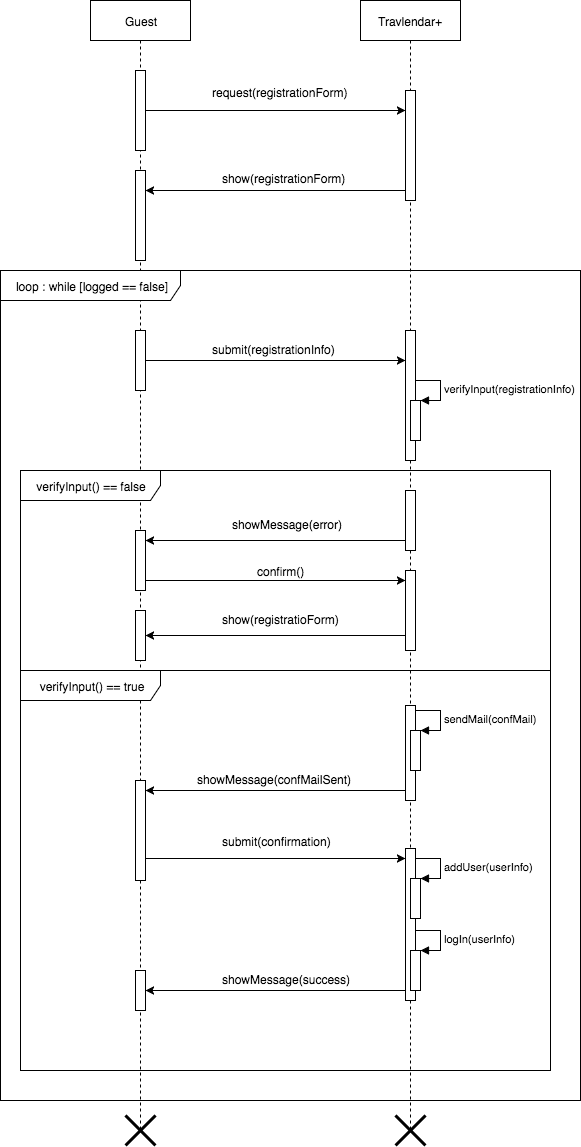
\includegraphics[width=0.69\textwidth]{SequenceDiagramSignup}
	\caption{Sign Up sequence diagram}
\end{figure}

\begin{figure}[H]
	\centering
	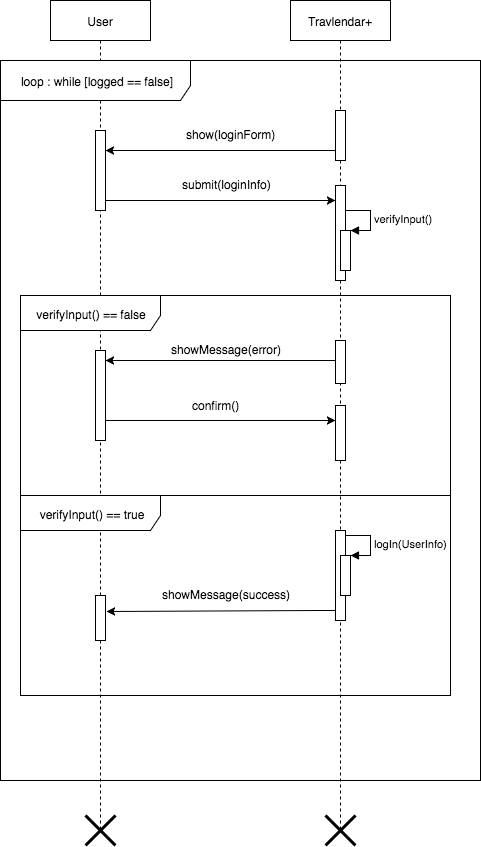
\includegraphics[width=0.8\textwidth]{SequenceDiagramLogin}
	\caption{Log In sequence diagram}
\end{figure}

\begin{figure}[H]
	\centering
	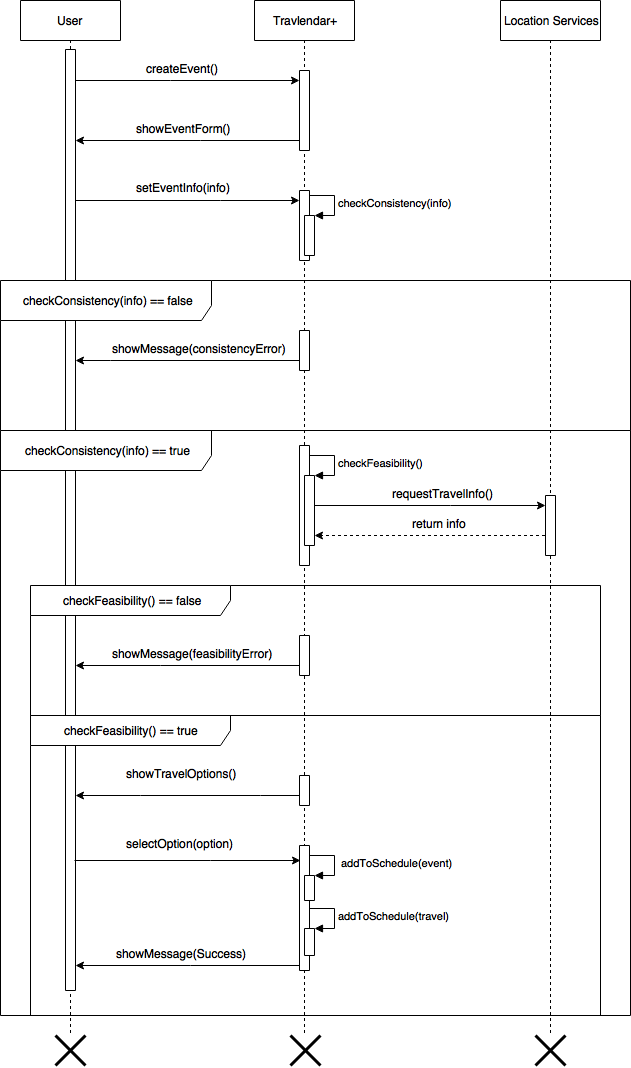
\includegraphics[width=0.8\textwidth]{SequenceDiagramEventCreation}
	\caption{Normal and Flexible event creation sequence diagram}
\end{figure}

\begin{figure}[H]
	\centering
	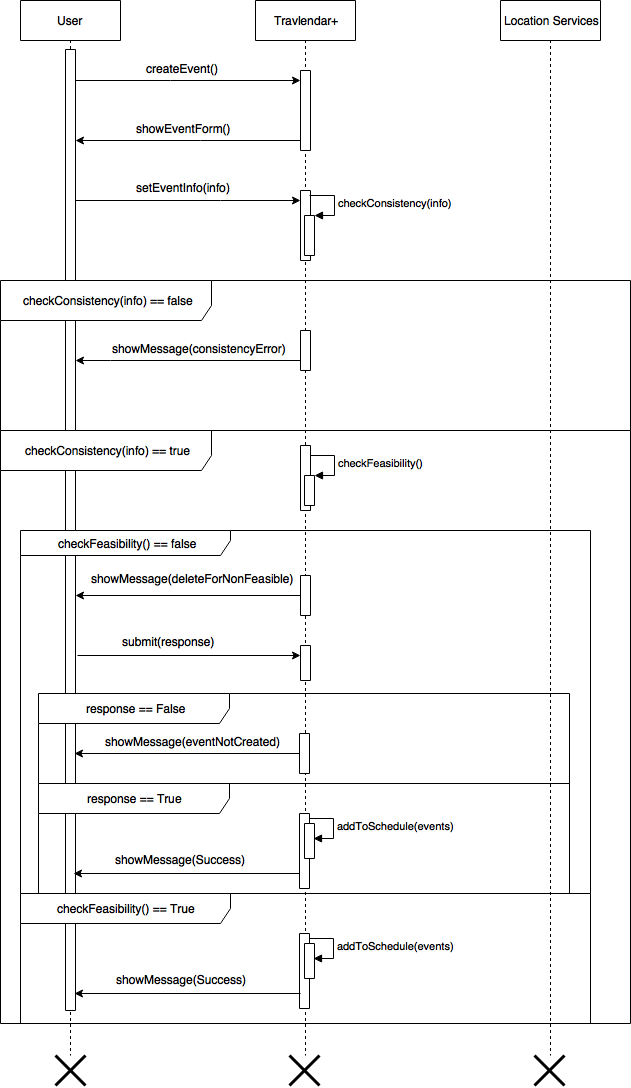
\includegraphics[width=0.8\textwidth]{SequenceDiagramRepetitiveEventCreation}
	\caption{Recurrent event creation sequence diagram}
\end{figure}


\begin{figure}[H]
	\centering
	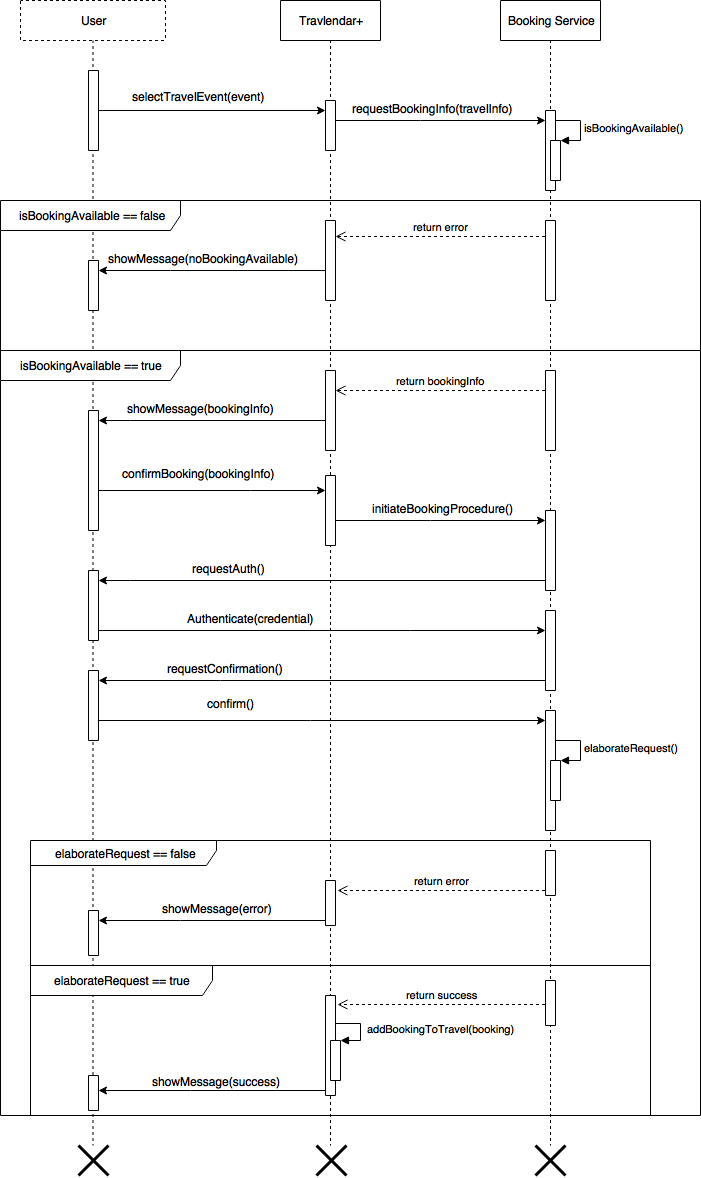
\includegraphics[width=0.8\textwidth]{SequenceDiagramTravelBooking}
	\caption{Travel booking sequence diagram}
\end{figure}

\newpage
\subsection{Product Functions}
In this section the most important features of the application are explained.

\begin{itemize}
	\item \textbf{Manage meetings}\\
	The System allows the User to add, edit and delete events in the schedule for a particular day. During the creation of the event, the User must specify the name of the event, the time and date of start and end of the event, the location of the event and the location from which it will be reached. Furthermore, the User will be able to add additional information about the event such as a briefly description and a category.\\
	For each event, the User is also provided with a list of possible travel means: the System will compute the best travel mean options accordingly with the information provided and the Users' travel preferences. The User will then be able to select one of the mean of transportation proposed.\\
	The User is also able to modify informations about a specific event or to delete it.\\
	The System guarantees the feasibility of the schedule for each day. To do this, it allows the User to add or edit only events in the schedule that are not in conflict with the ones already present.\\
	Finally, the User can choose to be notified a certain time before the event.
	
	
	\item \textbf{Set travel preferences}\\
	The User is able to customize his/her travel preferences globally activating or deactivating travel means that are:
	\begin{itemize}
		\item Personal motor vehicle
		\item Public transport
		\item Personal bicycle
		\item Taxi services
		\item Car sharing services
		\item Bike sharing services
		\item On foot
	\end{itemize} 
	Furthermore, for each travel mean a set of editable constraints is provided. The System gives also the possibility to activate an \textit{Eco Mode} option: in this case, the best travel solution will be computed in order to minimize carbon footprint.
	
	\item \textbf{Create flexible and repetitive events}\\
	The User is allowed to create flexible and repetitive events. Flexible events are particular type of events in which the User, besides the information about event date and location, must specify a window of time where the event can occur and a duration. In order to preserve the feasibility of the schedule, the System can arbitrarily move the event inside the window's bounds.\\
	On the other hand, repetitive events are particular type of events that are repeated with a frequency specified by the User. For these type of events, the User will be able to provide informations about start and end time and location, but will not be able to select a global travel means. For each occurrence of the event, the User will be allowed to request travel options and choose a travel mean.
	
	\item \textbf{Transport booking}\\
	The System provides a way to book some of the travel means proposed during the schedule phase relying on third party services. The User will be automatically redirected to the app or to the site of the service supplier to complete the purchase.
	However, the System provides only an interface for these services: the User might be requested to sign up/log in and to provide payment information in order to buy a ticket or book a ride. All the operations which occur in this phase are totally performed out of the application.
\end{itemize}

\subsection{User Characteristics}
\textit{Travlendar+} is suitable for all kind of Users, with no age limit.
We give for granted that both Users have access to Internet and are able to install and use the mobile application.\\
The characters are:
\begin{itemize}
	\item \textit{Guest:} a person who downloads and opens the app but still has to sign up. He/she cannot use any of the functions provided by \textit{Travlendar+}.
	\item \textit{User:} a registered User who has to log-in in order to access any feature of the application. He/she can retrieve his/her personal data from any device with the app installed just providing credentials.
	\item \textit{Logged-in User:} a User who logged in to the application and can manage his personal schedule, edit personal information and preferences. In order to book travels, he/she might need to be registered on third-party services.
\end{itemize}

\subsection{Constraints, Dependencies, Assumptions}
\textbf{Constraints}
\begin{itemize}
	\item Users are located in Milan.
	\item Users must have a smartphone equipped with an OS compatible with the application.  
	\item Users must have Internet connection.
	\item The System must ask Users for the permission to acquire, store and process personal data. Therefore, the System must offer the possibility to the Users to delete their personal account and the associated data.
\end{itemize}

\noindent \textbf{Dependencies}
\begin{itemize}
	\item The System will rely on external APIs to retrieve informations about travel means and associated ETA. 
	\item Travel booking options are provided by external third party services.
	\item The System needs a DBMS in order to store and retrieve Users' data.
\end{itemize}

\noindent \textbf{Assumptions}
\begin{itemize}
	\item \textbf{[D.1]} The given email is assumed to be correct.
	\item \textbf{[D.2]} The sent email is assumed to be correctly received.
	\item \textbf{[D.3]} The events informations provided by the user are correct.
	\item\textbf{[D.4]} Event time constraint are respected by the User.
	\item \textbf{[D.5]} The informations about the event are correct.
	\item \textbf{[D.6]} The informations about available mobility options and related travel time are correct.
	\item \textbf{[D.7]} If selected, the private means of transport are available without any delay.
	\item \textbf{[D.8]} The start location of the travel is known and correct.
	\item \textbf{[D.9]} All selected travel means specified in the preferences are potentially available to the User.
	\item \textbf{[D.10]} A minimum walking distance is assumed in order to reach every mean of transport. Such distance will not be taken into account unless significant with respect to the travel time, meaning unless it influences the ETA by more than a minute.
	\item \textbf{[D.11]} The User is registered to the service which offers the booking option.
	\item \textbf{[D.12]} The System internal clock time used to provide notifications is correct.
\end{itemize}
